% Edited: Removed code before and after figure section
% that was automatically knitted from the .Rmd
\begin{figure}
\centering
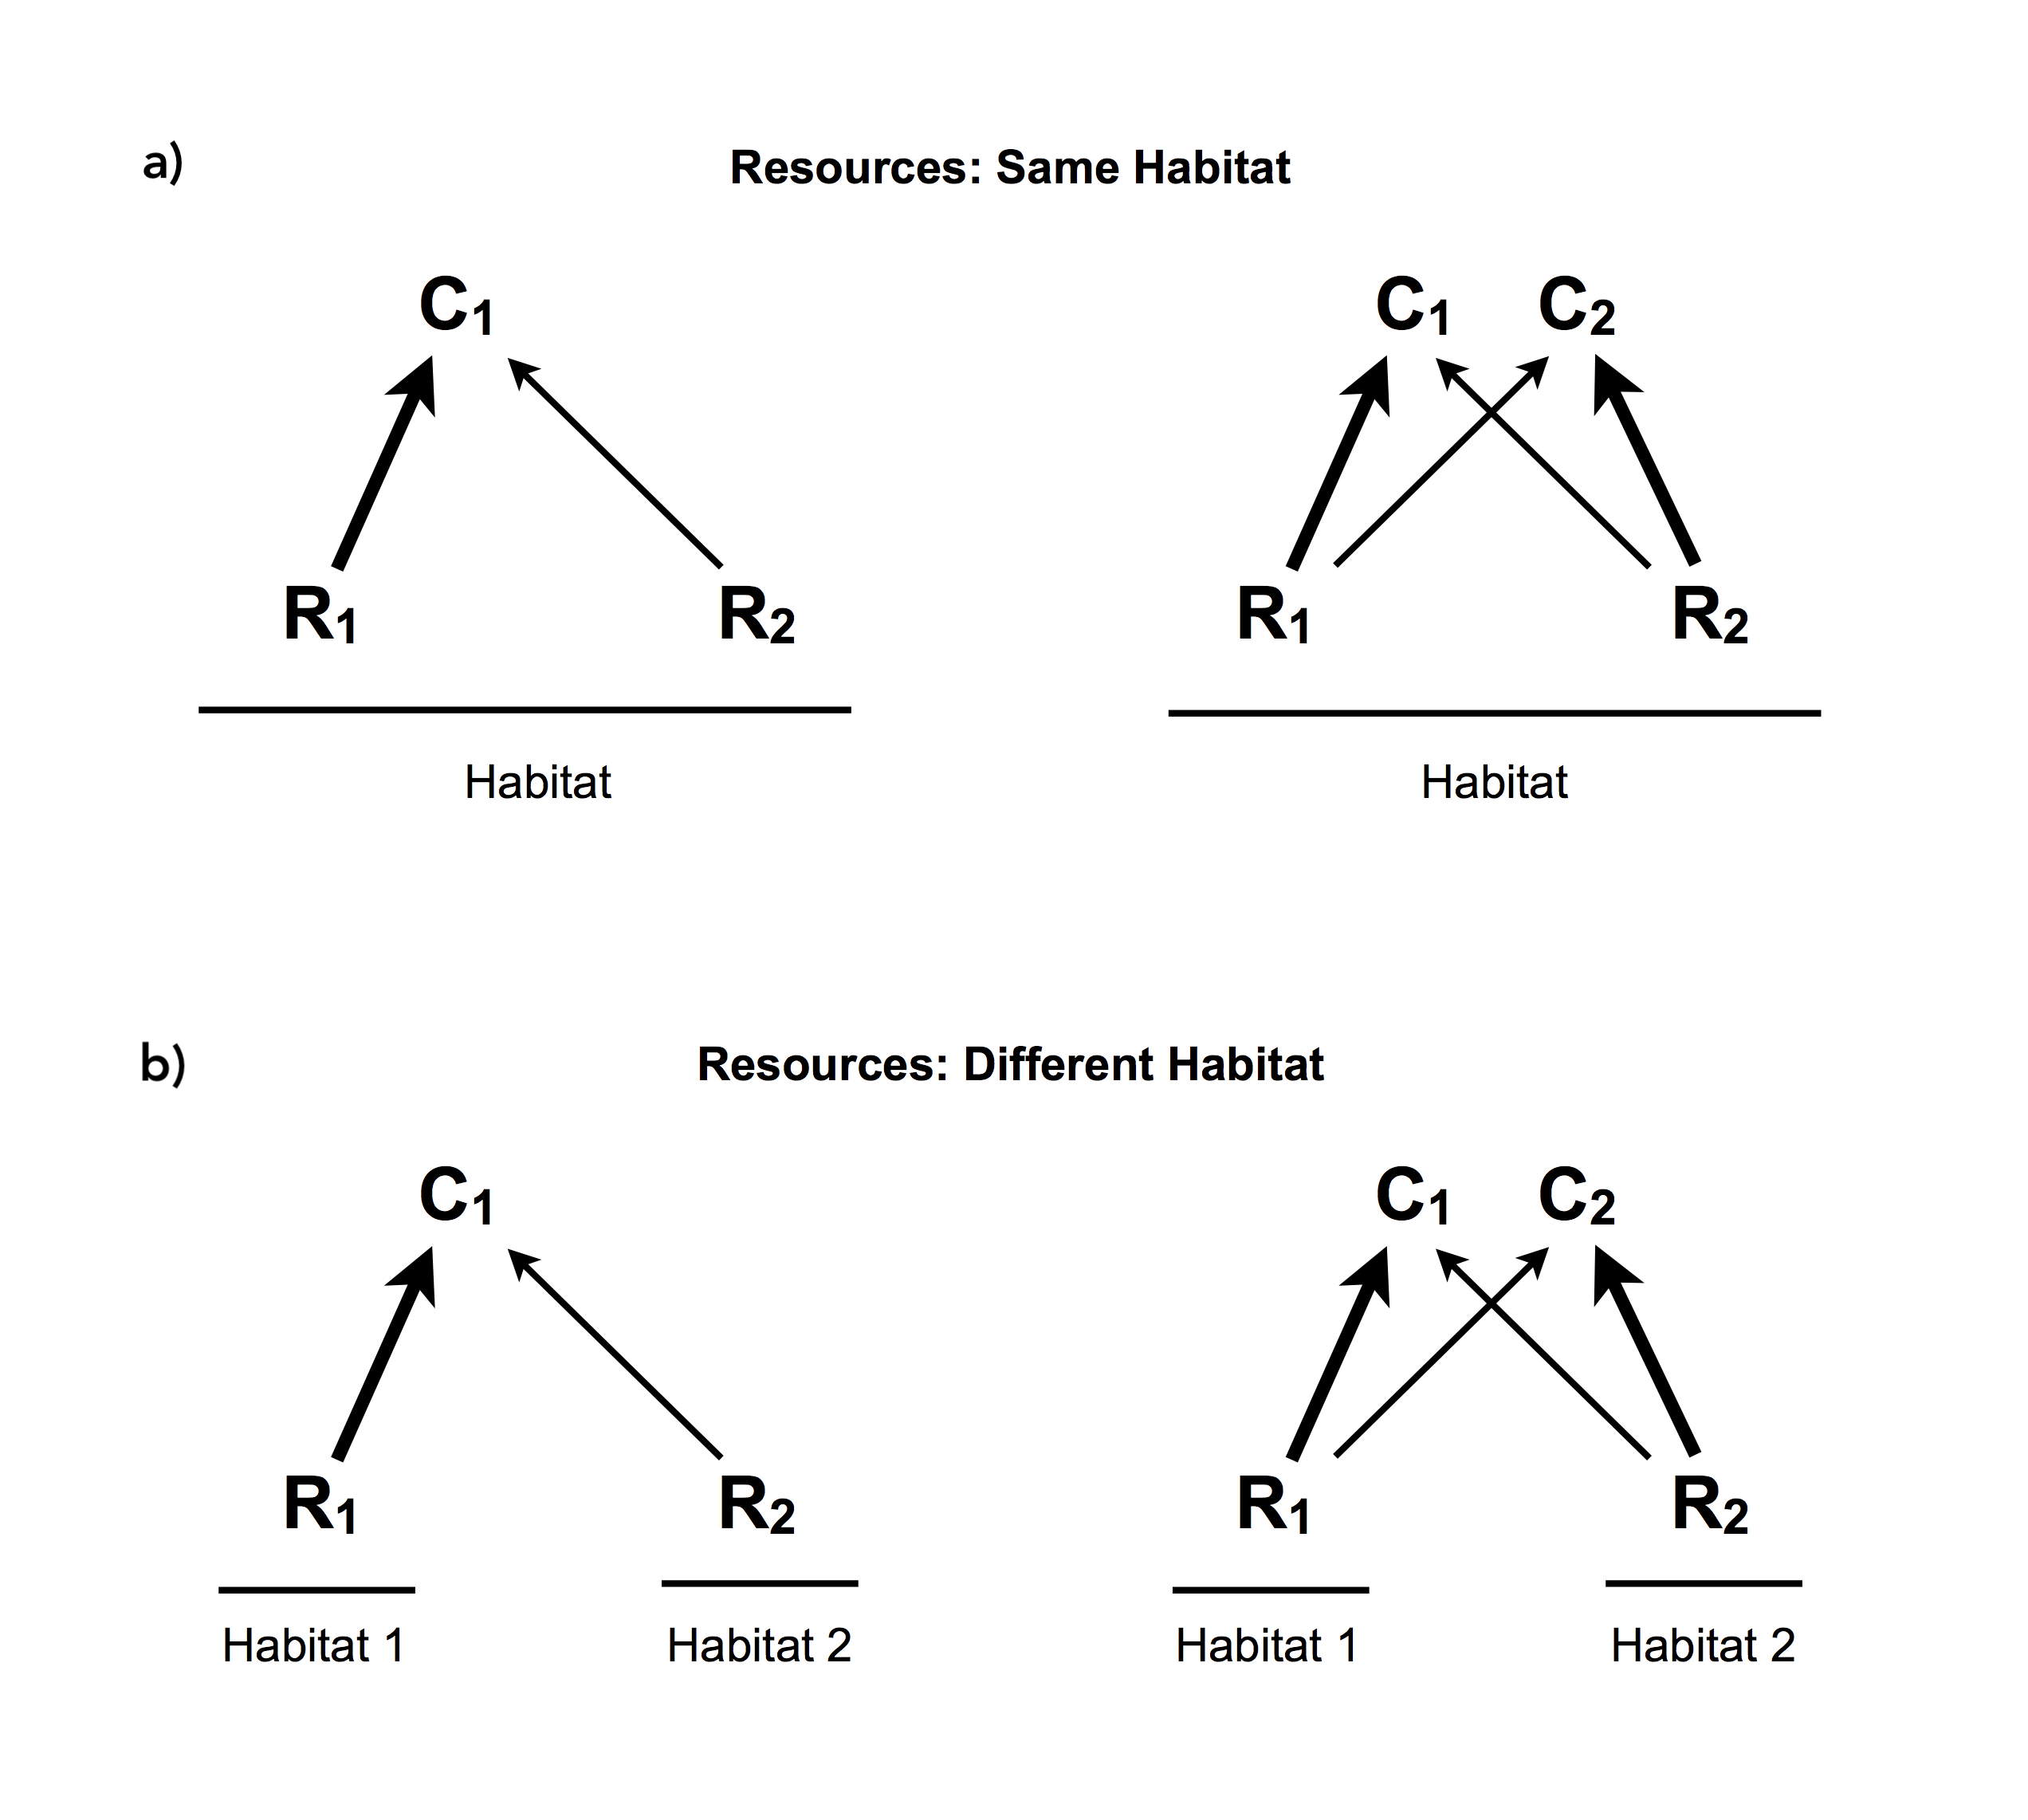
\includegraphics{Fig_1_ForagingScenarios}
\caption{\label{fig:foraging_scenarios}\textbf{Ecological foraging
scenarios.} I examined whether the effect of ecological character
displacement on food-web dynamics depended on whether consumers competed
for resources that occurred in the same (a) vs.~different habitats (b).
Note that inferences about character displacement can only be made by
comparing food webs with (right) and without (left) a competing
consumer, so I arbitrarily set \emph{C}\textsubscript{2} = 0 for these
comparisons. The width of each arrow corresponds to the initial attack
rate (\emph{a}\textsubscript{ij}) of consumer \emph{j} on resource
\emph{i}. Note that \emph{C}\textsubscript{1} was pre-adapted to
\emph{R}\textsubscript{1} (\emph{a}\textsubscript{11} \textgreater{}
\emph{a}\textsubscript{21}), while \emph{C}\textsubscript{2} was a
mirror image, being pre-adapted to \emph{R\textsubscript{2}}
(\emph{a}\textsubscript{22} = \emph{a}\textsubscript{11};
\emph{a}\textsubscript{12} = \emph{a}\textsubscript{21}). In each
scenario, I assumed consumer feeding rates increased linearly with
resource abundance. I also relax this assumption and consider a more
realistic functional response when resources occurred in different
habitats (b).}
\end{figure}

\begin{figure}
\centering
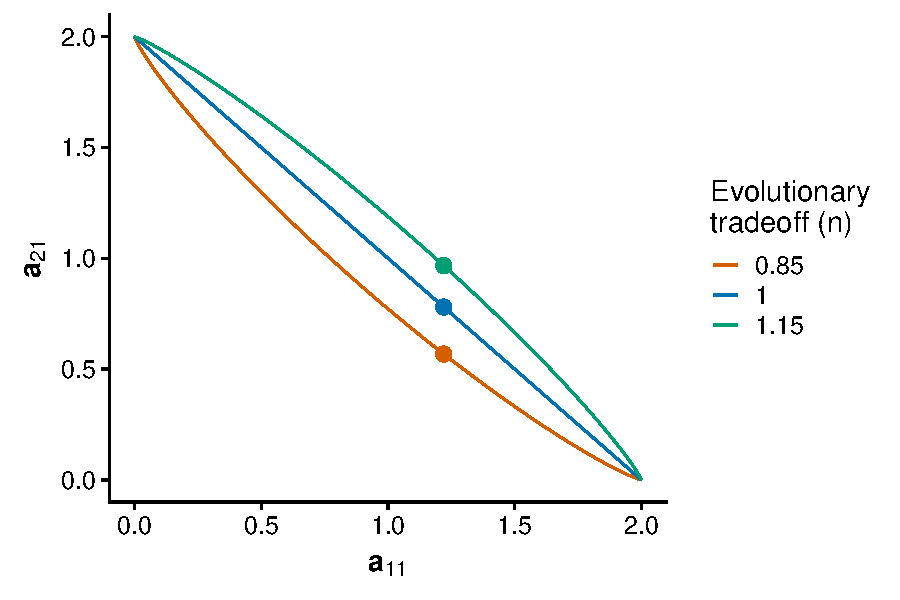
\includegraphics{Fig_2_Tradeoffs.pdf}
\caption{\label{fig:tradeoff}\textbf{Evolutionary tradeoffs in consumer
attack rates.} In each foraging scenario, I explored the effects of
three different tradeoffs: intermediate combinations of attack rates
(\emph{a}\textsubscript{1,\emph{j}}, \emph{a}\textsubscript{2,\emph{j}})
are higher than the extremes (green line, \emph{n} \textgreater{} 1);
extreme combinations of attack rates are higher than intermediate
investments (orange line, \emph{n} \textless{} 1); and all combinations
of attack rates have the same total attack rate (blue line, \emph{n} =
1). Points corresponding to attack rates at the beginning of the
simulation for \emph{C}\textsubscript{1}, which was pre-adapted to
\emph{R}\textsubscript{1} (\emph{a}\textsubscript{11} \textgreater{}
\emph{a}\textsubscript{12}). Note that \emph{C}\textsubscript{2} was a
mirror image of \emph{C}\textsubscript{1}, being pre-adapted to
\emph{R}\textsubscript{2} (\emph{a}\textsubscript{22} =
\emph{a}\textsubscript{11}; \emph{a}\textsubscript{12} =
\emph{a}\textsubscript{21}).}
\end{figure}

\begin{figure}
\centering
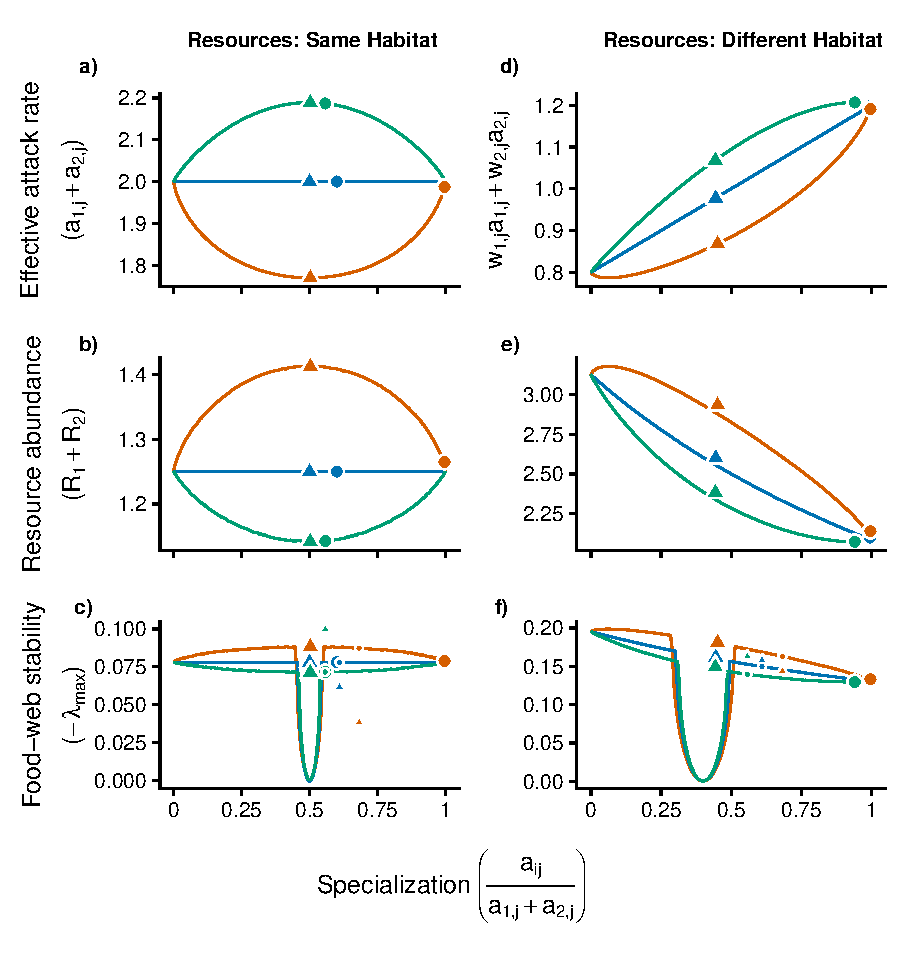
\includegraphics{Fig_3_MacArthur_LawlorSmith.pdf}
\caption{\label{fig:plot_fig3}\textbf{Effect of character displacement
on food-web dynamics under different evolutionary tradeoffs and foraging
scenarios.} Lines show predicted values when both consumers and
resources are present. Different line colors correspond to different
tradeoffs in attack rates (green, \emph{n} = 1.15; blue, \emph{n} = 1;
orange, \emph{n} = 0.85). Large circles (two consumers) and triangles
(one consumer) correspond to the end points of the eco-evolutionary
simulation for \emph{C}\textsubscript{1} (the choice to display
\emph{C}\textsubscript{1} was arbitrary), whereas as small shapes
correspond to the starting points (only in stability panels). In both
foraging scenarios, feeding rates increase linearly with resource
abundance, but the equation for the effective attack rate is different.}
\end{figure}

\begin{figure}
\centering
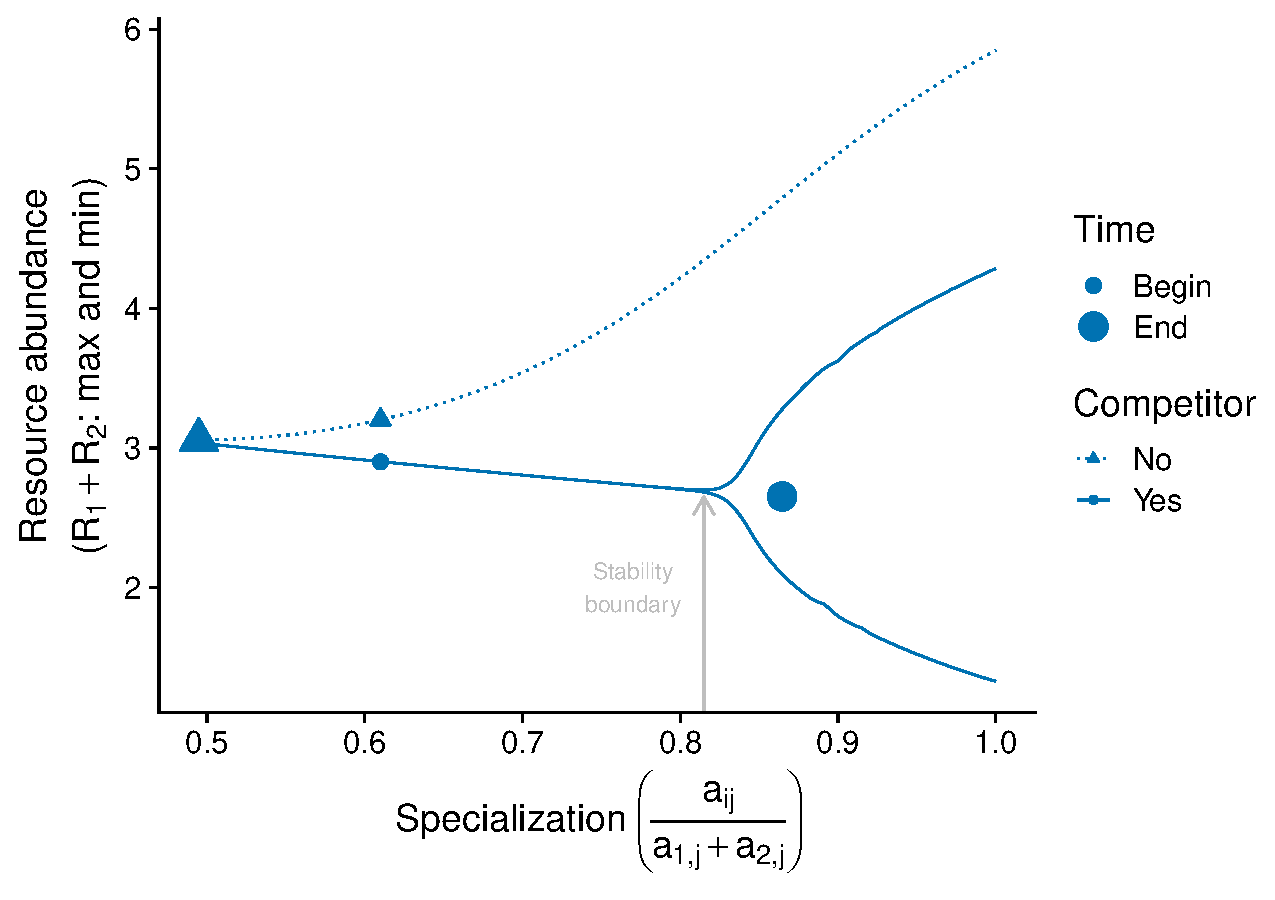
\includegraphics{Fig_4_Bifurcation.pdf}
\caption{\label{fig:bifur_plot}\textbf{Character displacement creates an
unstable food web}. Lines illustrate the effect of character
displacement across the range of specialization for
\emph{C}\textsubscript{1} (the choice to display
\emph{C}\textsubscript{1} was arbitrary), while the points are the
results of an eco-evolutionary simulation. Note that I increased the
total investment in attack rates (\emph{A} = 3.3) to create a scenario
that could result in an unstable food web. Although I specified a linear
tradeoff in attack rates for this simulation, different tradeoff shapes
do not qualitatively alter these results (see Appendix S4, Fig. S1).}
\end{figure}

